\section{函数列的收敛}
\label{sec:nspace-convergence-of-sequences}

有了具体的赋范函数空间，同一列函数就可以在几种意义下讨论收敛：每个输入处的值是否收敛，所有输入上的最大误差是否趋于零，积分误差是否趋于零，误差超过给定阈值的区域是否越来越小。把函数看作向量时，它们分别对应“逐分量”“最大分量”“加权和”和“超差分量的份额”。

有限维向量的这几种收敛等价，函数列的收敛方式之间却只有在附加条件下才能互相推出。第~\ref{chap:integration}章已经用逐点与几乎处处收敛建立了单调收敛和支配收敛定理，本节把这些收敛方式放在一起比较，并用一致可积性补上从依测度收敛到$L^1$收敛所需的条件。

本节固定测度空间$(X,\mathcal A,\mu)$与一列可测函数$f_n$及可测函数$f$，它们几乎处处取有限值。

\subsection{逐点、一致与\texorpdfstring{$L^p$}{Lp}收敛}
\label{sec:nspace-pointwise-uniform-lp}

逐点收敛与一致收敛是对函数本身的要求，第~\ref{chap:metric-space-maps}章已经定义：逐点收敛允许达到给定精度所需的序号依赖于$x$，一致收敛要求同一个序号对所有$x$有效。$L^p$收敛（$1\leq p<\infty$）则是$\lVert f_n-f\rVert_p\to0$，它只看误差$p$次幂的积分。

\paragraph{代表的选择}
这三种收敛对零测集的态度不同。逐点收敛和一致收敛是对选定的代表说的：把$f_n$在一个零测集上改值，可能破坏逐点收敛，也可能把一致收敛的序列变得不一致收敛。

所以在等价类上讨论时，应当改用两个说法。一是几乎处处收敛，即存在零测集$E$使$f_n(x)\to f(x)$对$x\notin E$成立；二是本质一致收敛，即$\lVert f_n-f\rVert_\infty\to0$。

$L^p$收敛和下一小节的依测度收敛只依赖等价类：改动零测集上的值不改变任何积分，也不改变任何集合的测度。

\paragraph{一致收敛推出\texorpdfstring{$L^p$}{Lp}收敛的条件}
一致收敛控制所有点上的误差，积分误差自然也受控制，但这需要总测度有限。若$\mu(X)<\infty$，由$\lvert f_n-f\rvert\leq\lVert f_n-f\rVert_\infty$几乎处处成立，取$p$次幂后积分，得到
\begin{equation}
 \lVert f_n-f\rVert_p\leq\mu(X)^{1/p}\,\lVert f_n-f\rVert_\infty ,
 \label{eq:nspace-uniform-to-lp}
\end{equation}
所以本质一致收敛推出每个$L^p$收敛。测度无限时这一推论失败。在$\mathbb R$上取Lebesgue测度与$h_n=\tfrac1n\mathbf 1_{[0,n]}$，则
\[
 \lVert h_n\rVert_\infty=\frac1n\to0,\qquad \lVert h_n\rVert_1=1.
\]
高度在降低，支撑却在扩大，总面积不变。

不同指数之间也有类似的比较，同样依赖有限测度。设$\mu(X)<\infty$，$1\leq p<r<\infty$。对$\lvert h\rvert^p\cdot1$用Hölder不等式，指数取$r/p$及其共轭指数$r/(r-p)$，得到
\[
 \int_X\lvert h\rvert^p\,d\mu\leq\Bigl(\int_X\lvert h\rvert^r\,d\mu\Bigr)^{p/r}\mu(X)^{1-p/r}.
\]
两边开$p$次方，整理成
\begin{equation}
 \lVert h\rVert_p\leq\mu(X)^{1/p-1/r}\lVert h\rVert_r.
 \label{eq:nspace-lp-inclusion}
\end{equation}
取$h=f_n-f$，$L^r$收敛推出$L^p$收敛。把式~\eqref{eq:nspace-lp-inclusion}看作包含映射$L^r\to L^p$的有界性，是第~\ref{chap:linear-operators}章的内容。

\paragraph{三个对照序列}
图~\ref{fig:nspace-convergence-modes}与表~\ref{tab:nspace-convergence-modes}对照了$[0,1]$上Lebesgue测度下的三个序列，它们标出了各收敛方式之间不能互推的边界。

\begin{BookInlineFigure}
  \centering
  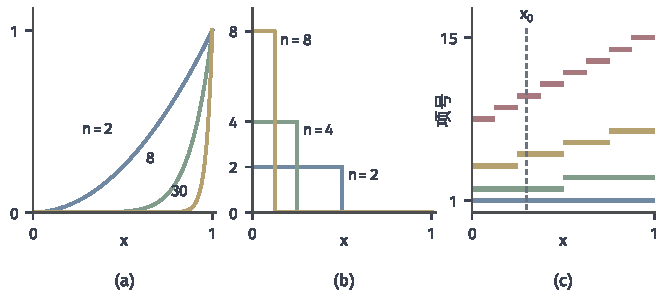
\includegraphics[width=112mm]{figures/04-spaces-measures-and-geometry/03-function-spaces/matplotlib/nspace-convergence-modes/figure.pdf}
  \caption{三种收敛方式的反例。(a)$x^n$，$n=2,8,30$：除$x=1$外逐点趋于$0$，$L^p$范数趋于零，最大误差恒为$1$。(b)窄尖峰$n\mathbf 1_{(0,1/n)}$，$n=2,4,8$：每一点最终为零，积分恒为$1$。(c)打字机序列的前$15$项，第$k$层（$k=0,1,2,3$，蓝、绿、黄、红）把$[0,1)$等分为$2^k$段；纵轴为项号，横条为支撑，竖虚线$x=x_0$在每一层恰好穿过一个横条。}
  \label{fig:nspace-convergence-modes}
\end{BookInlineFigure}

\begin{BookInlineTable}
  \centering
  \begin{tabular}{@{}lccc@{}}
    \toprule
    序列 & 逐点收敛到$0$ & $L^1$收敛到$0$ & 一致收敛到$0$ \\
    \midrule
    $x^n$ & 除$x=1$外 & 是 & 否 \\
    $n\mathbf 1_{(0,1/n)}$ & 是（处处） & 否 & 否 \\
    打字机序列 & 处处不收敛 & 是 & 否 \\
    \bottomrule
  \end{tabular}
  \caption{$[0,1]$上Lebesgue测度下三个序列的收敛性质。}
  \label{tab:nspace-convergence-modes}
\end{BookInlineTable}

先看$x^n$。它的$L^p$范数为
\[
 \lVert x^n\rVert_p=(np+1)^{-1/p}\to0.
\]
逐点极限在$x=1$处为$1$、其余处为$0$。单点零测，所以作为$L^p$中的元素，逐点极限与零元素相同，两种说法并不矛盾。最大误差恒为$1$，不一致收敛。

再看窄尖峰$g_n=n\mathbf 1_{(0,1/n)}$。对$x>0$，只要$n>1/x$就有$g_n(x)=0$，所以处处收敛到$0$。但积分的值不变：
\[
 \lVert g_n\rVert_1=n\cdot\frac1n=1.
\]
逐点收敛允许不同位置在不同时刻进入误差带，因而管不住越来越窄、越来越高的峰。即使总测度有限，逐点收敛也推不出$L^p$收敛。

\begin{example}[打字机序列]
\label{ex:nspace-typewriter}
对$k=0,1,2,\ldots$与$j=0,\ldots,2^k-1$，令
\[
 h_{k,j}=\mathbf 1_{[j2^{-k},(j+1)2^{-k})},
\]
按$k$从小到大、同一层内按$j$从小到大排成一列$h_{0,0},h_{1,0},h_{1,1},h_{2,0},\ldots$。第$k$层每一项的范数为
\[
 \lVert h_{k,j}\rVert_p=2^{-k/p},
\]
随项号增大趋于零，所以序列在每个$L^p$（$p<\infty$）中收敛到$0$。

但对每个$x_0\in[0,1)$，每一层恰好有一项在$x_0$处取$1$，其余项取$0$。所以数列$(h_{k,j}(x_0))$中$0$和$1$都出现无穷多次，在任何一点都不收敛。$L^p$收敛推不出逐点收敛，也推不出几乎处处收敛。
\end{example}

打字机序列虽然整列不逐点收敛，定理~\ref{thm:nspace-lp-ae-subsequence}却保证它有几乎处处收敛的子列。这里可以直接写出一个：子列$h_{k,0}=\mathbf 1_{[0,2^{-k})}$对每个$x>0$在$2^{-k}<x$后恒为零，所以在$(0,1]$上逐点收敛到$0$，例外只有零测点$x=0$。

\subsection{依测度收敛}
\label{sec:nspace-convergence-in-measure}

逐点收敛逐个检查位置，$L^p$收敛累计误差的大小。还有一种更粗的要求：不管误差具体多大，只问误差超过某个阈值的区域有多大。用向量的语言说，它只看超差分量所占的份额。

\begin{definition}[依测度收敛]
\label{def:nspace-convergence-in-measure}
若对每个$\varepsilon>0$，
\begin{equation}
 \lim_{n\to\infty}\mu\bigl(\{x:\lvert f_n(x)-f(x)\rvert>\varepsilon\}\bigr)=0,
 \label{eq:nspace-convergence-in-measure}
\end{equation}
称$f_n$\term{依测度收敛}（convergence in measure）到$f$。
\end{definition}

定义只控制“大误差出现的范围”，不管大误差有多大，也不管它出现在哪里。窄尖峰$n\mathbf 1_{(0,1/n)}$依测度收敛到$0$：对任意$\varepsilon>0$，超差集合至多是$(0,1/n)$，测度$1/n\to0$。它的$L^1$误差却恒为$1$，所以依测度收敛推不出$L^1$收敛。打字机序列的第$k$层超差集合是一个长为$2^{-k}$的区间，同样依测度收敛到$0$，而它处处不逐点收敛。

\paragraph{\texorpdfstring{$L^p$}{Lp}收敛推出依测度收敛}
积分误差小，大误差所占的区域就小。对$1\leq p<\infty$与$\varepsilon>0$，在超差集合$A_n=\{\lvert f_n-f\rvert>\varepsilon\}$上有$\lvert f_n-f\rvert^p>\varepsilon^p$，所以
\begin{equation}
 \varepsilon^p\mu(A_n)\leq\int_{A_n}\lvert f_n-f\rvert^p\,d\mu\leq\lVert f_n-f\rVert_p^p .
 \label{eq:nspace-chebyshev}
\end{equation}
这是\term{Chebyshev不等式}（Chebyshev inequality）。若$\lVert f_n-f\rVert_p\to0$，则$\mu(A_n)\to0$，即依测度收敛。这一推论不要求测度有限。

取$p=1$，用$[0,1]$上的三角形$h(x)=1-\lvert2x-1\rvert$走一遍，$\varepsilon=\tfrac12$。超差集合是$A=(\tfrac14,\tfrac34)$，$\mu(A)=\tfrac12$，式~\eqref{eq:nspace-chebyshev}的两边是
\[
 \varepsilon\,\mu(A)=\frac14,\qquad \lVert h\rVert_1=\frac12.
\]
图~\ref{fig:nspace-chebyshev}显示了这个不等式的来源：高为$\varepsilon$、宽为$\mu(A)$的矩形完全落在曲线下方。

\begin{BookInlineFigure}
  \centering
  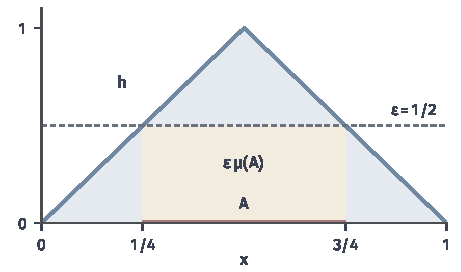
\includegraphics[width=78mm]{figures/04-spaces-measures-and-geometry/03-function-spaces/matplotlib/nspace-chebyshev/figure.pdf}
  \caption{Chebyshev不等式，取$h(x)=1-\lvert2x-1\rvert$、$\varepsilon=\tfrac12$。红线是超差集合$A=(\tfrac14,\tfrac34)$，黄色矩形面积$\varepsilon\,\mu(A)=\tfrac14$，含于面积为$\lVert h\rVert_1=\tfrac12$的蓝色区域之内。}
  \label{fig:nspace-chebyshev}
\end{BookInlineFigure}

\paragraph{有限测度下几乎处处收敛推出依测度收敛}
几乎处处收敛说每一点（零测集之外）迟早进入误差带，依测度收敛说没进入误差带的区域在缩小。在有限测度空间中，前者推出后者。

\begin{theorem}[几乎处处收敛推出依测度收敛]
\label{thm:nspace-ae-to-measure}
设$\mu(X)<\infty$，$f_n\to f$几乎处处。则$f_n$依测度收敛到$f$。
\end{theorem}

\begin{proof}
固定$\varepsilon>0$，令
\[
 B_N=\bigcup_{n\geq N}\{\lvert f_n-f\rvert>\varepsilon\},
\]
它随$N$单调下降。若$x\in\bigcap_NB_N$，则有无穷多个$n$使$\lvert f_n(x)-f(x)\rvert>\varepsilon$，$f_n(x)$不收敛到$f(x)$。所以$\bigcap_NB_N$含于不收敛点的集合，是零测集。

$\mu(B_1)\leq\mu(X)<\infty$，由测度的上连续性，
\[
 \mu(B_N)\to\mu\Bigl(\bigcap_NB_N\Bigr)=0.
\]
而$\{\lvert f_N-f\rvert>\varepsilon\}\subseteq B_N$，所以它的测度也趋于零。
\end{proof}

上连续性要求$\mu(B_1)<\infty$，有限测度正是用在这里。测度无限时结论失败：在$\mathbb R$上取Lebesgue测度与$f_n=\mathbf 1_{[n,n+1]}$，每一点在$n>x$后都有$f_n(x)=0$，处处收敛到$0$；但$\mu(\{f_n>\tfrac12\})=1$，不依测度收敛。

\paragraph{依测度收敛列的几乎处处收敛子列}
依测度收敛推不出几乎处处收敛，打字机序列就是例子。但和$L^p$收敛一样，总可以抽出一个几乎处处收敛的子列。

\begin{theorem}[依测度收敛的子列]
\label{thm:nspace-measure-subsequence}
设$f_n$依测度收敛到$f$。则存在子列$(f_{n_k})$，使$f_{n_k}\to f$几乎处处。
\end{theorem}

\begin{proof}
由定义，可以递归地取$n_1<n_2<\cdots$，使$E_k=\{\lvert f_{n_k}-f\rvert>2^{-k}\}$满足$\mu(E_k)<2^{-k}$。令$F_j=\bigcup_{k\geq j}E_k$，则
\[
 \mu(F_j)\leq\sum_{k\geq j}2^{-k}=2^{1-j}.
\]
若$x\notin F_j$，则对所有$k\geq j$有$\lvert f_{n_k}(x)-f(x)\rvert\leq2^{-k}$，所以$f_{n_k}(x)\to f(x)$。

于是不收敛的点都落在$\bigcap_jF_j$中，而$\mu(\bigcap_jF_j)\leq\mu(F_j)\leq2^{1-j}$对每个$j$成立，这个集合是零测集。
\end{proof}

证明的想法是挑选超差集合测度可求和的子列，使“无穷多次超差”的点只能组成零测集。这里没有用到测度有限。结合Chebyshev不等式，它也给出了定理~\ref{thm:nspace-lp-ae-subsequence}的另一个证明。

\subsection{一致可积性}
\label{sec:nspace-uniform-integrability}

窄尖峰依测度收敛到$0$，$L^1$误差却恒为$1$：峰越来越窄，但越来越高，积分始终集中在测度趋零的区域上。要从依测度收敛得到$L^1$收敛，需要防止积分躲进小区域里的大取值中。第~\ref{chap:integration}章的支配收敛定理用一个共同的可积上界做到这一点；一致可积性是更弱、却恰好够用的条件。本小节设$\mu(X)<\infty$。

\begin{definition}[一致可积]
\label{def:nspace-uniform-integrability}
设$\mu(X)<\infty$，$\{f_n\}\subseteq L^1(\mu)$。若
\begin{equation}
 \lim_{M\to\infty}\ \sup_{n}\int_{\{\lvert f_n\rvert>M\}}\lvert f_n\rvert\,d\mu=0,
 \label{eq:nspace-uniform-integrability}
\end{equation}
称$\{f_n\}$\term{一致可积}（uniformly integrable）。
\end{definition}

对单个可积函数$f$，总有
\[
 \int_{\{\lvert f\rvert>M\}}\lvert f\rvert\,d\mu\to0\qquad(M\to\infty).
\]
这是因为被积函数$\lvert f\rvert\mathbf 1_{\{\lvert f\rvert>M\}}$被$\lvert f\rvert$控制，且在$\lvert f\rvert<\infty$的点处当$M\to\infty$时趋于零，由支配收敛定理即得。一致可积要求这件事对整族函数以同样的速度发生，即大取值区域上的积分一致地小。

\paragraph{尖峰与共同上界}
窄尖峰不是一致可积的。对任意$M$，当$n>M$时$\{g_n>M\}=(0,1/n)$，其上的积分为$1$，所以
\[
 \sup_n\int_{\{g_n>M\}}g_n\,d\mu=1
\]
不随$M$趋于零。这正是它不$L^1$收敛的原因。

把峰的高度从$n$压到$\sqrt n$，情况就变了。令$f_n=\sqrt n\,\mathbf 1_{(0,1/n)}$，只有$\sqrt n>M$时$\{f_n>M\}$才非空，其上的积分为
\[
 \int_{\{f_n>M\}}f_n\,d\mu=\sqrt n\cdot\frac1n=\frac1{\sqrt n}<\frac1M.
\]
上确界不超过$1/M$，所以这一族一致可积。图~\ref{fig:nspace-uniform-integrability}并排画出这两族函数。

\begin{BookInlineFigure}
  \centering
  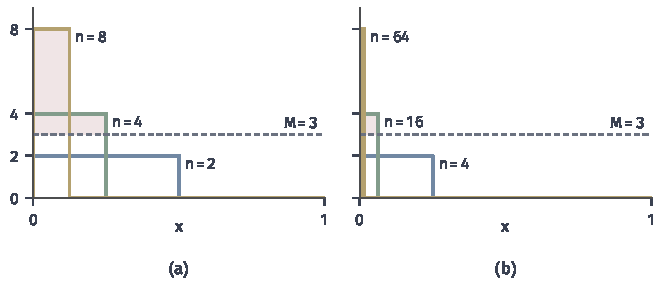
\includegraphics[width=112mm]{figures/04-spaces-measures-and-geometry/03-function-spaces/matplotlib/nspace-uniform-integrability/figure.pdf}
  \caption{尖峰的一致可积性，阈值$M=3$，浅红色为函数高于$M$的部分。(a)$g_n=n\mathbf 1_{(0,1/n)}$，$n=2,4,8$：每个高于阈值的尖峰，整根矩形的面积都是$1$，阈值抬高也不变。(b)$f_n=\sqrt n\,\mathbf 1_{(0,1/n)}$，$n=4,16,64$：高度相同的情况下宽度小得多，$\{f_n>M\}$上的积分是$1/\sqrt n$，随$n$变小。}
  \label{fig:nspace-uniform-integrability}
\end{BookInlineFigure}

有共同可积上界的族总是一致可积的。若$\lvert f_n\rvert\leq G$几乎处处对所有$n$成立，$G\in L^1$，则$\{\lvert f_n\rvert>M\}\subseteq\{G>M\}$，
\[
 \sup_n\int_{\{\lvert f_n\rvert>M\}}\lvert f_n\rvert\,d\mu\leq\int_{\{G>M\}}G\,d\mu\to0.
\]
窄尖峰没有这样的上界：$\sup_ng_n(x)$在$x\in[\tfrac1{n+1},\tfrac1n)$上等于$n>\tfrac1x-1$，不可积。

\paragraph{一致的小区域控制}
一致可积的族在小区域上的积分也一致地小，这是下面证明要用的形式。对任意可测集$A$与$M>0$，把$A$分成$\lvert f_n\rvert>M$与$\lvert f_n\rvert\leq M$两部分，得到
\begin{equation}
 \int_A\lvert f_n\rvert\,d\mu\leq\int_{\{\lvert f_n\rvert>M\}}\lvert f_n\rvert\,d\mu+M\mu(A).
 \label{eq:nspace-ui-small-sets}
\end{equation}

给定$\eta>0$，先取$M$使第一项对所有$n$都小于$\eta/2$，再令$\delta=\eta/(2M)$，则$\mu(A)<\delta$时$\sup_n\int_A\lvert f_n\rvert\,d\mu<\eta$。取$A=X$还得到$\sup_n\lVert f_n\rVert_1\leq\eta/2+M\mu(X)<\infty$，一致可积的族在$L^1$中有界。

\paragraph{从依测度收敛到\texorpdfstring{$L^1$}{L1}收敛}
有了小区域上的一致控制与$L^1$有界性，就可以把依测度收敛加强为$L^1$收敛：大误差区域的测度趋于零，一致可积保证这些区域上的积分也趋于零。

\begin{theorem}[依测度收敛与一致可积推出\texorpdfstring{$L^1$}{L1}收敛]
\label{thm:nspace-vitali}
设$\mu(X)<\infty$，$\{f_n\}\subseteq L^1(\mu)$一致可积，且$f_n$依测度收敛到可测函数$f$。则$f\in L^1(\mu)$，且$\lVert f_n-f\rVert_1\to0$。
\end{theorem}

\begin{proof}
先证$f$可积。由定理~\ref{thm:nspace-measure-subsequence}，有子列$f_{n_k}\to f$几乎处处。由Fatou引理与上面的$L^1$有界性，
\[
 \int_X\lvert f\rvert\,d\mu\leq\liminf_{k\to\infty}\int_X\lvert f_{n_k}\rvert\,d\mu\leq\sup_n\lVert f_n\rVert_1<\infty.
\]

再估计误差。给定$\varepsilon>0$与$\eta>0$，令$A_n=\{\lvert f_n-f\rvert>\varepsilon\}$。在$A_n$之外误差不超过$\varepsilon$，在$A_n$上用三角不等式，所以
\[
 \int_X\lvert f_n-f\rvert\,d\mu\leq\varepsilon\,\mu(X)+\int_{A_n}\lvert f_n\rvert\,d\mu+\int_{A_n}\lvert f\rvert\,d\mu.
\]

对族$\{f_n\}$取上一段的$\delta_1$；单个可积函数$f$构成的族$\{f\}$也一致可积，对它取$\delta_2$。依测度收敛给出$N$，使$n\geq N$时$\mu(A_n)<\min(\delta_1,\delta_2)$，此时后两项都小于$\eta$。于是$n\geq N$时
\[
 \lVert f_n-f\rVert_1\leq\varepsilon\,\mu(X)+2\eta.
\]
$\varepsilon,\eta$任意，故$\lVert f_n-f\rVert_1\to0$。
\end{proof}

证明把误差分成两部分：在误差不超过$\varepsilon$的区域上，贡献至多$\varepsilon\mu(X)$；误差超过$\varepsilon$的区域测度趋零，依测度收敛只保证这一点，其上的积分则由一致可积控制。有限测度用在两处：$\varepsilon\mu(X)$有限，以及式~\eqref{eq:nspace-ui-small-sets}给出$L^1$有界。

用前面的例子验证。$f_n=\sqrt n\,\mathbf 1_{(0,1/n)}$一致可积，又依测度收敛到$0$，定理给出$\lVert f_n\rVert_1\to0$；直接计算也得到$\lVert f_n\rVert_1=1/\sqrt n\to0$。窄尖峰不满足一致可积，定理不能用，结论也确实不成立。

\paragraph{回到支配收敛}
若$f_n\to f$几乎处处，且$\lvert f_n\rvert\leq G\in L^1$，则在有限测度下，定理~\ref{thm:nspace-ae-to-measure}给出依测度收敛，上面的论证给出一致可积，于是定理~\ref{thm:nspace-vitali}推出$\lVert f_n-f\rVert_1\to0$。这就回到了第~\ref{chap:integration}章的支配收敛定理。

共同可积上界只是一致可积的充分条件。一致可积只要求大取值区域上的积分一致地小，允许没有共同可积上界的族。

反过来，在有限测度下，$L^1$收敛的序列一定一致可积。证明要把前面的小区域控制转回大取值集合，篇幅较长，读者可查阅测度论的教材。所以在有限测度下，一致可积恰好刻画了依测度收敛何时能升级为$L^1$收敛。
